% Straight up stealing preamble from Eli Holmes 
%%%%%%%%%%%%%%%%%%%%%%%%%%%%%%%%%%%%%%START PREAMBLE THAT IS THE SAME FOR ALL EXAMPLES
\documentclass{article}

%Required: You must have these
\usepackage{Sweave}
\usepackage{graphicx}
\usepackage{tabularx}
\usepackage{hyperref}
\usepackage{natbib}
%\usepackage[backend=bibtex]{biblatex}
%Strongly recommended
  %put your figures in one place
 
%you'll want these for pretty captioning
\usepackage[small]{caption}

\setkeys{Gin}{width=0.8\textwidth}  %make the figs 50 perc textwidth
\setlength{\captionmargin}{30pt}
\setlength{\abovecaptionskip}{0pt}
\setlength{\belowcaptionskip}{10pt}
% manual for caption  http://www.dd.chalmers.se/latex/Docs/PDF/caption.pdf

%Optional: I like to muck with my margins and spacing in ways that LaTeX frowns on
%Here's how to do that
 \topmargin -1.5cm        
 \oddsidemargin -0.04cm   
 \evensidemargin -0.04cm  % same as oddsidemargin but for left-hand pages
 \textwidth 16.59cm
 \textheight 21.94cm 
 %\pagestyle{empty}       % Uncomment if don't want page numbers
 \parskip 7.2pt           % sets spacing between paragraphs
 %\renewcommand{\baselinestretch}{1.5} 	% Uncomment for 1.5 spacing between lines
\parindent 0pt% sets leading space for paragraphs
\usepackage{setspace}
%\doublespacing

%Optional: I like fancy headers
\usepackage{fancyhdr}
\pagestyle{fancy}
\fancyhead[LO]{How do climate change experiments actually change climate}
\fancyhead[RO]{2016}
 
%%%%%%%%%%%%%%%%%%%%%%%%%%%%%%%%%%%%%%END PREAMBLE THAT IS THE SAME FOR ALL EXAMPLES

%Start of the document
\begin{document}

% \SweaveOpts{concordance=TRUE}
 \bibliographystyle{/Users/aileneettinger/citations/Bibtex/styles/nature.bst}
\title{How do climate change experiments actually change climate?} % Paper 1/Large group paper from Reconciling Experimental and Observational Approaches for Climate Change Impacts

\author{A. K. Ettinger,I. Chuine, B. Cook, J. Dukes, A. Ellison, M. Johnston, A.M. Panetta,\\ C. Rollinson, Y. Vitasse, E. Wolkovich}
%\date{\today}
\maketitle  %put the fancy title on
%\tableofcontents      %add a table of contents
%\clearpage
%%%%%%%%%%%%%%%%%%%%%%%%%%%%%%%%%%%%%%%%%%%%%%%%%%%

\section* {Aim}

The aim is to write a Concept/Synthesis Paper, for Nature Climate Change, about maximizing benefits of field-based climate change experiments. We argue that there is a need to improve our understanding of how climate is actually altered by these experiments, particularly if we wish to use these experiments to forecast biological impacts of climate change. %yann: perhaps also to determine which methods of warming alter the least other climatic variables or to define the most appropriate method regarding the focus of the study (phenology, growth, survival etc)?%annmarie: Somewhere in this paper,  we should discuss that is important that “how” climate variables are modified relative to the predicted change under various emission scenarios is important.  Thus, the “how” should be not only the direction and magnitude of the variable change but also the extent to which the change mirrors change projected for the region in which the experiment took place). build up a discussion of studies that report only mean shifts in temperature in the intro. 

\section* {Introduction}
\par Future climate change is expected to cause dramatic alterations to Earth's biota. The physiology, distribution, and abundance of organisms will shift, and likely cause cascading community and ecosystem effects \citep{thomas2004,parmesan2006,sheldon2011,urban2012}. Much uncertainty remains,however, about how particular individuals, populations, communities, and ecosystems will respond, making predicting organism responses to the climate change one of the most significant challenges facing biology today.
% EMW: See quick (could be much better) changes below to better handle temperature and precipitation in this paragraph. Much work is on temperature because that's a known, relatively easy to predict effect, at least when compared to precipitation (we may or may not want to sneak this in). 
\par One way that people have sought to understand and forecast future biological conditions is through in situ experimental climate manipulations. Many studies have focused on manipulations to replicate expected higher temperatures. Commonly used field techniques for this include passive warming, such as open-top chambers, and active warming methods, including forced air, soil cables,infra-red radiation. Active warming methods are the most controlled, consistent, and ``true to climate change predictions" \citep{kimball2005,kimball2008,aronson2009,wolkovich2012}, and we therefore focus on these methods here. Recently, interest has also expanded to understand changing precipitation. Today, many active warming methods are frequently combined with precipitation manipulations, including drought, snow-removal, and supplemental precipitation treatments, in an effort to create climatic conditions such as those forecasted under future climate change scenarios \citep{price1998,cleland2006,sherry2007,rollinson2012}.
\par Experimental in situ climate manipulations with active warming offer several advantages over other approaches, such as long-term observational data and growth chamber studies for understanding biological impacts of climate change. These experiments allow effects of temperature and precipitation to be isolated from other environmental changes. In addition, a range of warming and/or precipitation treatments can be applied, such that potential non-linear relationships of climate responses can be evaluated. These advantages come at a cost, however. Experimental in situ climate manipulations are logistically challenging and expensive \citep{aronson2009}. It is difficult to design, implement, and monitor replicated experiments that consistently apply the intended climate manipulations.  
\par As we seek to prepare for future, altered conditions in our biological environment, scientists and others often wish to extrapolate the results of in situ climate change experiments to forecast how organisms and ecosystems will respond to particular climate change scenarios. Even in cases where this is not the explicit goal of warming and other climate change experiments, it would be incredibly useful to be able to apply knowledge gained from these experiments to improve our understanding and forecasting of how anthropogenic warming will affect species' performance (growth, survival) and distributions. Our ability to make this application is currently limited because a detailed assessment of exactly how experimental warming treatments alter climate, beyond the typically reported mean differences, and the extent to which these manipulations accurately model the real world, both present and future, is lacking. 
\par Here, we suggest that a more nuanced understanding of how climate change experiments actually change climate is critical if we wish to realize the forecasting potential of climate change experiments. We first use plot-level microclimate data from 12 climate change experiments that manipulate temperature (and precipitation, in some cases), while monitoring daily temperature and other climate vairables, to demonstrate the complex ways that climate is altered by active warming treatments, both directly and indirectly. The data we use are from experiments in North America and Europe that were collected between 1991 and 2014, and have been merged into a new, publicly available database (see Supplemental Materials for details). We then discuss the challenges of interpreting biological implications of experimental shifts in climate, when these climate manipulations are more complex then simple shifts in the mean. Finally, we make recommendations for future climate change experiments.

\section* {Complications in extrapolating experimental climate change}
Climate change experiments often include detailed monitoring of climate variables at the plot level, yielding large amounts of data, such as daily or hourly temperature and other climate variables, over the course of the experiment. However, biologists are generally interested primarily in the biological responses associated with each treatment (e.g. growth, abundance, or phenology of a species). Not surprisingly, then, authors typically provide detailed information on the observed biological responses, and report only the mean change in climate over the course of the experiment and whether or not that mean change matched their target level of change \citep{price1998,clark2014a,clark2014b,rollinson2012}. The imposed climate manipulations result in much more than a simple shift in the mean, however. The magnitude of change experienced by organisms in these manipulations is likely to vary in time and space, and the equipment required to conduct these manipulations can also alter climate at the plot level. 
\subsection* {Treatments vary over time}
The common practice of reporting only the mean temperature difference, across the duration of the study, may hide variations in annual, seasonal, and daily minimum and maximum temperatures.There are frequently strong seasonal variations in experimental warming effects (Figure 1). This can occur because treatments are not applied consistently over the year, either because heat applications are frequently shut off during some seasons such as when snow cover is present \citep[e.g.][]{clark2014a,clark2014b} (Yann and Isabelle- could you recomend some studies from Europe that also use this methodology) or because some heating methods, even if left on throughout the year, are not capable of applying consistent warming year-round (e.g. infrared radiation, CITATION- Christy, Yann, and/or Jeff could you suggest 1 or 2?). Furthermore, seasonal precipitation patterns can alter the effectiveness of warming treatments (CITATION- Christy, Yann, and/or Jeff could you suggest 1 or 2?). % it is likely that this would yield different effects than if heating were turned on during winter (because then you change soil nutrient mineralization which might be important in winter and so change nutrient availability and moisture for the growing season ).
\par In addition to seasonal patterns, experimental warming effects can vary widely across longer timescales, such as among years (Figure 2). This is probably due to interactive effects of warming treatments and other aspects of weather that may vary annually. For example, Hoepner and Dukes (2012) found that infrared heaters failed to achieve the target temperatures during rainstorms. 
\par Warming treatments can also vary on shorter timescales, such as within a day. This often leads to a decrease in the diurnal temperature range within experimental plots, compared with ambient conditions \citep{hoeppner2012}. This may be similar to what is projected for parts of world \citep{ipcc2013}. However, this will likely vary spatially, as some regions have experienced higher daytime warming than nighttime warming, whereas others have experienced the opposite\citep{ipcc2013}. 
\par A detailed comparison of projections versus observations in climate change experiments is lacking. Thus, it is unknown how divergent these annual, seasonal, and daily variations may be from real (i.e. non-experimental) climate patterns.  %there are several recent papers showing the importance of diurnal over nocturnal temperature on phenology.
\par Anne Marie- please write a paragraph on your suggested discussion "that 3-5 year studies may not capture ultimate, long-term responses that may actually be in the opposite direction to short-term responses.  Cite recent Global Change Biology paper by Harte et al.  Ideally, we want to run studies long enough to capture population-level responses to warming." I would love to work this in and I think you are the one to write it!
\subsection* {Treatments vary in space}
In addition to temporal variation, there can be spatial variation in experimental warming effects, such that extrapolation of experimental warming to forecast climate change impacts may not be a straightforward space-for-time substitution. For example, we used three studies that used a blocked design to examine spatial variation in the amount of warming (i.e. the difference between treatment and control plots within a block). We found that the amount of warming may vary by more than one degree among blocks (Figure 2, Table 1).
\par Presumably, there will be spatial variation in future climate change effects, given that warming to date has varied spatially \citep{ipcc2013}).  Accurate extrapolation of climate change experiments may therefore depend on the extent to which experiments encompass a representative amount of existing natural variation (e.g. gradients in slope, aspect, etc) present at the scale at which the extrapolation is being made. An added complication is that inferences made from space-for-time substitutions are frequently invalidated, when they have been tested with empirical evidence \citep{johnson2008}. When experimental manipulations aimed at understanding future responses are imposed in a spatially varying environment, we need to be explicit about what assumptions are made in this modified space-for-time substution, think critically about whether these assumptions are realistic, and then carefully interpret results in light of these assumptions. (Aaron- do you think we need more here about space-for-time substition and its problems? If so, what? or do you have citations we should add?). There is also documented small-scale variation in the amount of warming, within experimental plots, atleast from passive warming studies \citep {marion1997}.

\subsection* {Experimental infrastructure alters climate}
The experimental structures themselves alter temperature and other important biotic and abiotic variables, in ways that are not generally examined or reported in experimental warming studies. The possible existence of these effects are widely acknowledged, and some studies include "shams" or "disturbance controls" to account for them. However, the magnitude of structural effects on climate are rarely discussed or interpreted in climate change studies.
\par To investigate the magnitude of these effects, we compared temperature and soil moisture data from four active warming studies at two sites: Duke Forest and Harvard Forest\citep{farnsworth1995,clark2014a, marchin2015, pelini2011}. These were the only studies in our database that included two types of control plots: structural controls (i.e. ``shams" or ``disturbance controls," which contained all the warming infrastructure, such as soil cables or infrared heating units but with no heat applied) and ambient controls with no infrastructure added (see Supplemental Materials for details).  
\par We were surprised to find that experimental structures altered air and soil temperatures in opposing ways:  air temperatures were higher in the structural controls, compared with the ambient air with no structures installed, whereas soil temperatures were lower in the structural controls compared with ambient soil (Figure 3). This was consistent across the different temperature models we fit (mean, minimum, and maximum), and the sign of the effects was consistent across study-sites and months, although the magnitude varied among sites (Table 3) and across seasons (Figure 3). Soil moisture was lower in structural controls compared with ambient conditions (Figure 1S). In addition to these documented effects, experimental structures may alter conditions by creating shade, intercepting precipitation, and altering herbivory and other biotic interactions. Further documentation and analysis of the effects of these experimental structures on abiotic and biotic factors, as well as in depth interpretation of how these effects may alter focal variables, is an important next step for climate change experimentation, particularly if we wish to apply results to forecasting.
\section* {Secondary effects of climate change manipulations}
Climate change experiments often manipulate one or two climate variables, such as temperature and precipitation. However, as scientists who have conducted these experiments have likely experienced, climatic variables are nearly impossible to completely isolate from one another.  Temperature, for example, interacts with precipitation to alter the abiotic environment; Rollinson et al (2012) observed that a twenty percent increase in precipitation reduced mean hourly temperatures by 0.3 degrees Celsius over the course of their two-year experiment. Ideally, experimentally induced changes in other variables would be realistic; for example, the experimental treatment should not decrease moisture in an area projected to get wetter. At the very least, it is important to quantify the secondary effects of applied manipulations.  
\par Precipitation treatments typically reduce temperatures in climate change manipulations, as described above \citep[e.g.][]{sherry2007,rollinson2012}, but the magnitude of this effect can vary in space and time (Figure 2S). Experimental warming  reduces vapor pressure deficit and soil water content \citep[e.g. Figure 3S][]{sherry2007,morin2010,templer2016}. The magnitude of these effects are also likely to vary in space and time. 
\par Warming and precipitation treatments can also alter community composition, which is likely to have additional secondary effects. For example, tree composition shifted after three years of warming and modified precipitation treatments \citep{rollinson2012}. These shifts in composition may change competitive dynamics and, in turn, affect resource levels.  It can be difficult to tease out limiting resources and abiotic and biotic drivers of biological responses, but understanding the effects of an experimental treatment on these interrelated variables is critical when trying to determine mechanistic explanations for observed responses to warming.
\section* {Biological implications}
\par We have highlighted a suite of factors that complicate   interpretation of warming experiments. We argue that these largely unintended alterations are important for scientists to fully understand and report in their research because they are likely to have biological implications (Figure 4).
\par Climate change experiments may affect phenology in complicated ways, for example. Plant phenology is likely to be altered in opposing ways by the increased air temperatures and decreased soil moisture characterized by warming treatments. Indeed, these opposing drivers may be responseible for the observed discrepancy between observational and experimental phenology responses to warming\citep{wolkovich2012}. In addition, plant phenology responds to minimum temperatures, as well as mean and maximuma, and this may also play a role in the discrepency between observational and experimental studies \citep{shen2016,matthews2016}. Lizzie, Aaron, Yann, Isabelle-Please recommend other citations for this!
\par Plant growth is also likely to be altered in opposing ways by the increased air temperatures and decreased soil moisture levels in experimentally warmed plots. For example, with warming and decreased VPD, stomata closure may reduce sapflow and growth \citep{templer2016}. Even small shifts in temperature may have a big effect, since the photosynthetic response to temperature is nonlinear \citep{berry1980}.
\par Direct and indirect effects of climate change experiments are also likely to affect soil respiration in ways that may alter net mineralization and therefore have other cascading effects. Yann: please add a few sentences and citations here!

\par Other biotic interactions are also likely to be affected by direct and indirect affects of climate change treatments. For example, Hoeppner and Dukes  (2012) found that rodent disturbancevaried by warming treatment (as well as year) in their climate change experiment. Aaron, Anne-Marie, Yann, and/or Jeff- please add other examples (with citations) if you can think of some good ones? A critical question is the extent to which these shifts in biotic interactions (and their effects on focal repsonses) are accurate forecasts of future shifts that are likely to occur with climate change, or due to side-effects that are unlikely to occur outside of experimental systems.
\section* {Recommendations for future climate change experiments}
 \par The complications of climate change experiments that  we describe are not meant to be criticisms or to imply that experimental climate change studies are not worthwhile. On the contrary, we believe that climate change experiments provide invaluable information about biological responses to climate change. We believe that we need to more fully explore the ways in which these climate change experiments are actually altering climate. Below we describe a few recommendations to improve implementation, interpretation, and communication of future climate change experiments.
\par\textit{Design realistic manipulations} by consulting climate change projections for the study region, and selecting warming and precipitation treatment methods that most accurately mimic anticipated changes. When it is not possible to match anticipated changes in climate, studies should report how imposed treatments compared to projected changes. In addition, the timing of these treatments should be carefully considered and ideally should match forecasts. If it is not possible to apply continuous treatments throughout the study, the seasonality and timing of treatments should be explicitly reported.
\par\textit{Include both structural and ambient controls} and collect, use, and report data collected within them. This will facilitate separating mechanisms due to experimental design from mechanisms due to actual shifts in climate.  
\par\textit{Maximize the length of climate change experiments} by running them for as long as possible. This will allow study of how inter-annual variations interact with climate change treatments, especially when looking at non-linear and multiyear processes such as phenology. It will also allow us to understand how long-term responses may differ from  transient ones. Citations, anyone?
\par\textit{Collect fine-scale climate data}, at least twice daily, and ideally hourly, to allow for minimum and maximum values to be analyzed and interpreted, in addition to mean values.
 \par\textit{Publish high quality, usable data and metadata} such that data can easily be shared and used by others. In the metadata, report the number and cause of missing data points for climate, especially those collected in warming treatments. (For example, are data missing because the heaters went out, or because rodents at the sensors?) Report the timing of applied warming treatments (i.e. exact start and end dates, within and across years), as well as variations in daytime and nighttime and seasonal variations in climate variables. 
\par\textit{Consider implementing and following community standards for reporting climate data} Do we have community standards for climate data? Ben- do you have any ideas of resources for this?
When studying biological implications of a global challenge as large as climate change, it facilitate progress if we can design, run, and report experiments in such a way that we can eventually create global dataset. This recommendation stems from our work gathering and analyzing data from many climate change experiments. We found that studies report a diverse range of climate variables, collected in different ways (i.e. soil temperature collected at different depths; soil moisture using different units and methods). It has been difficult to synthesize these data in a comprensive way that can fully address important questions. 
\par I would love someone to suggest points to make and/or take a stab at writing a closing paragraph!
\bibliography{/Users/aileneettinger/citations/Bibtex/mylibrary}
\section* {Tables}

\section* {Tables}
\par
% latex table generated in R 3.2.4 by xtable 1.8-2 package
% Wed Sep 21 23:07:18 2016
\begin{table}[ht]
\centering
\begin{tabular}{lrrr}
  \hline
 & Chisq & Df & Pr($>$Chisq) \\ 
  \hline
(Intercept) & 861.834 & 1.000 & 0.000 \\ 
  temptreat & 431.799 & 3.000 & 0.000 \\ 
  block & 5.795 & 2.000 & 0.055 \\ 
  temptreat:block & 43.094 & 6.000 & 0.000 \\ 
   \hline
\end{tabular}
\caption{Effects of warming vary by block, as summarized by a linear mixed effects model of mean soil temperatures, with year and site as nested random effects} 
\end{table}\par
% latex table generated in R 3.2.4 by xtable 1.8-2 package
% Wed Sep 21 23:07:18 2016
\begin{table}[ht]
\centering
\begin{tabular}{lrrr}
  \hline
 & Chisq & Df & Pr($>$Chisq) \\ 
  \hline
(Intercept) & 1455.294 & 1.000 & 0.000 \\ 
  temptreat & 126.093 & 3.000 & 0.000 \\ 
  year & 16.676 & 1.000 & 0.000 \\ 
  temptreat:year & 61.646 & 3.000 & 0.000 \\ 
   \hline
\end{tabular}
\caption{Effects of warming vary by year, as summarized by a linear mixed effects model of mean soil temperatures, with year and site as nested random effect} 
\end{table}\section* {}
\par
[1] exp10 exp08 exp04 exp03 exp07
12 Levels: exp01 exp02 exp03 exp04 exp05 exp06 exp07 exp08 exp09 ... exp12\par
% latex table generated in R 3.2.4 by xtable 1.8-2 package
% Wed Sep 21 23:07:22 2016
\begin{tabular}{rrr}
  \hline
Estimate & Std. Error & t value \\ 
  \hline
12.674 & 1.632 & 7.766 \\ 
  -0.356 & 0.092 & -3.859 \\ 
   \hline
\end{tabular}\par Summary of linear mixed effects model testing difference in mean air temperatures of structural controls compared with ambient controls (i.e.with no control chambers or warming infrastructure in place). The model included a fixed effect of control type and an intercept-only random effect of studysite to account for study and measurement, as well as environmental, differences.
\par
% latex table generated in R 3.2.4 by xtable 1.8-2 package
% Wed Sep 21 23:07:22 2016
\begin{tabular}{rrrr}
  \hline
 & Estimate & Std. Error & t value \\ 
  \hline
(Intercept) & 11.312 & 1.366 & 8.283 \\ 
  temptreatambient & 0.425 & 0.068 & 6.285 \\ 
   \hline
\end{tabular}\par Summary of linear mixed effects model testing difference in mean soil temperature (at the shallowest depth measured) of structural controls compared with ambient controls. The model included a fixed effect of control type and an intercept-only random effect of studysite to account for study and measurement, as well as environmental, differences.
\par
% latex table generated in R 3.2.4 by xtable 1.8-2 package
% Wed Sep 21 23:07:22 2016
\begin{tabular}{rrr}
  \hline
Estimate & Std. Error & t value \\ 
  \hline
7.161 & 1.381 & 5.186 \\ 
  -0.389 & 0.092 & -4.236 \\ 
   \hline
\end{tabular}\par Summary of linear mixed effects model testing difference in minimum air temperatures of structural controls compared with ambient controls (i.e.with no control chambers or warming infrastructure in place). The model included a fixed effect of control type and an intercept-only random effect of studysite to account for study and measurement, as well as environmental, differences.
\par
% latex table generated in R 3.2.4 by xtable 1.8-2 package
% Wed Sep 21 23:07:22 2016
\begin{tabular}{rrr}
  \hline
Estimate & Std. Error & t value \\ 
  \hline
10.493 & 1.334 & 7.866 \\ 
  0.346 & 0.068 & 5.089 \\ 
   \hline
\end{tabular}\par Summary of linear mixed effects model testing difference in minimum soil temperature (at the shallowest depth measured) of structural controls compared with ambient controls. The model included a fixed effect of control type and an intercept-only random effect of studysite to account for study and measurement, as well as environmental, differences.
\par
% latex table generated in R 3.2.4 by xtable 1.8-2 package
% Wed Sep 21 23:07:22 2016
\begin{tabular}{rrr}
  \hline
Estimate & Std. Error & t value \\ 
  \hline
18.187 & 1.899 & 9.576 \\ 
  -0.322 & 0.098 & -3.290 \\ 
   \hline
\end{tabular}\par Summary of linear mixed effects model testing difference in maximum air temperatures of structural controls compared with ambient controls (i.e.with no control chambers or warming infrastructure in place). The model included a fixed effect of control type and an intercept-only random effect of studysite to account for study and measurement, as well as environmental, differences.
\par
% latex table generated in R 3.2.4 by xtable 1.8-2 package
% Wed Sep 21 23:07:22 2016
\begin{tabular}{rrr}
  \hline
Estimate & Std. Error & t value \\ 
  \hline
13.599 & 1.670 & 8.145 \\ 
  0.572 & 0.076 & 7.532 \\ 
   \hline
\end{tabular}\par Summary of linear mixed effects model testing difference in maximum soil temperature (at the shallowest depth measured) of structural controls compared with ambient controls. The model included a fixed effect of control type and an intercept-only random effect of studysite to account for study and measurement, as well as environmental, differences.
\par
\section* {Figures}

 \begin{figure}[p]
     \centering
 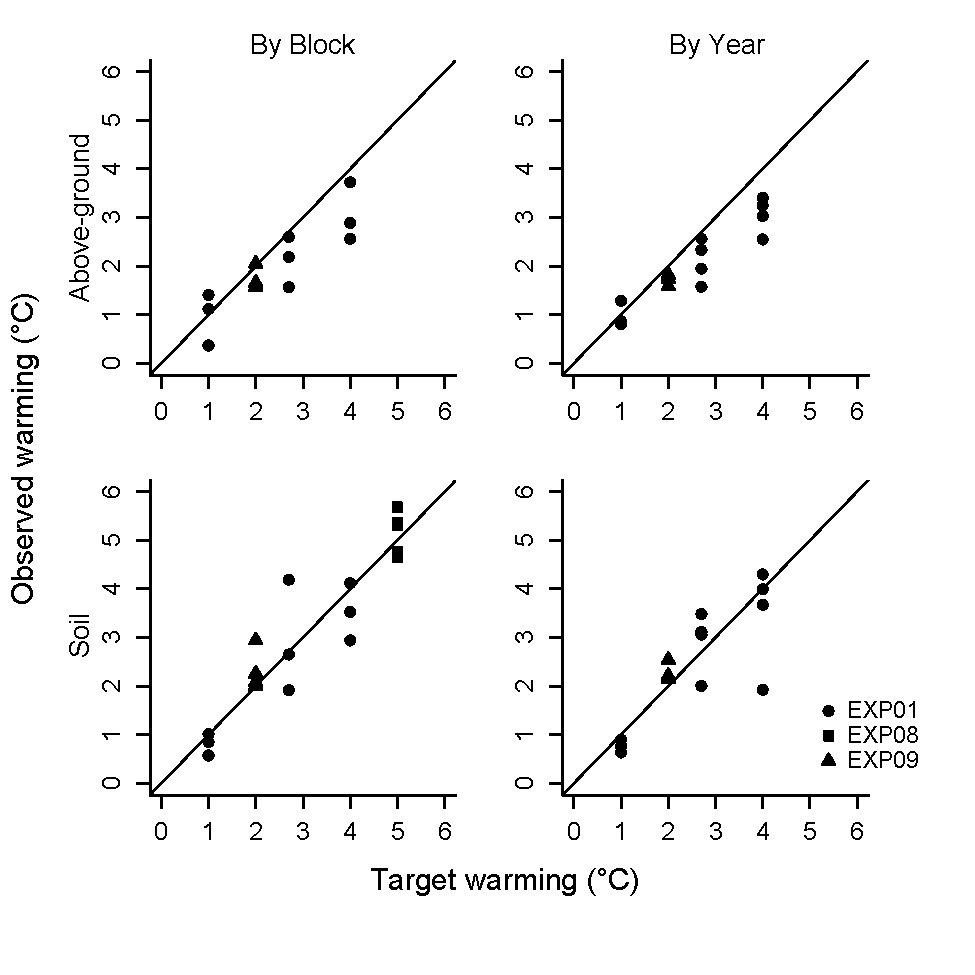
\includegraphics{../figures/BothWarmingbyblockyear.pdf}    
 \caption{The amount of warming (i.e. the difference between treatment and control plots, within each block) varies among blocks (left panels), as well as among years (right panels). See Tables 1 and 2 for statistical differences.}
 \end{figure}

 \begin{figure}[p]
     \centering
 \includegraphics{../figures/Exploratory_TimeSeries_SoilTemp1Mean_Deviation.png}    
 \caption{Time series of deviations from mean soil temperature over one year, in control (black line) and warming treatments with various target warming levels at 10 study sites.}
 \end{figure}

 \begin{figure}[p]
     \centering
 \includegraphics{../figures/ShamVSAmbient_mean.pdf}    
 \caption{Difference between mean air and soil temperatures in structural controls compared with ambient controls, with no control chambers or warming infrastructure in place. Air temperatures were higher, whereas soil temperatures were lower in the structural controls compared with ambient conditions. We show fixed effects from a mixed effects model that accounts for differences in experimental design and other factors among sites by including site as an intercept-only random effect (see Supplemental Materials for details). }
 \end{figure}
 \begin{figure}[p]
     \centering
 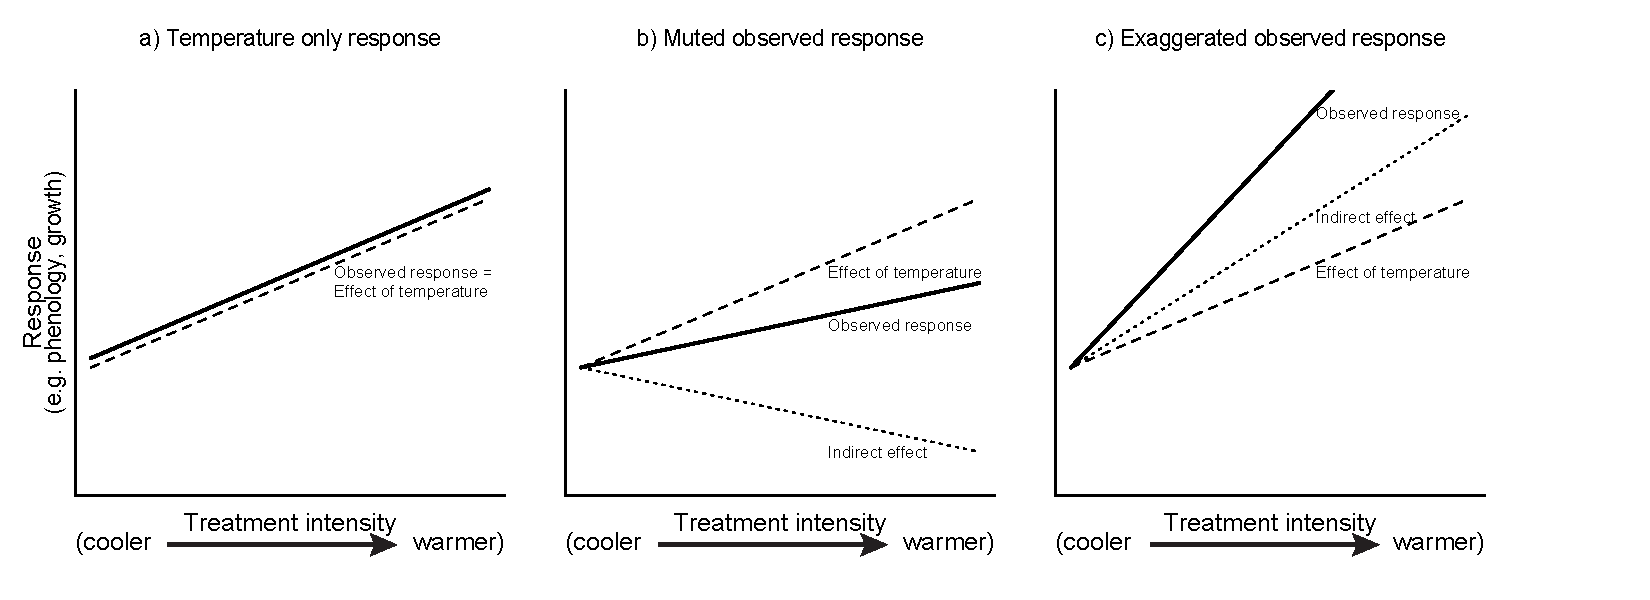
\includegraphics{../figures/DirIndWarmingEffects.pdf}    
 \caption{Experimental warming may cause biological responses to be muted or exaggerated, compared to direct responses to temperature alone, when indirect effects of experimental warming are also drivers of focal responses. For example, phenology may appear to be less sensitive to warming in experiments versus observational studies \citep{wolkovich2012} because experimental warming reduces soil moisture, perhaps more than natural warming.}
 % EMW: Change the Y axis title so it's clearer -- effect of structural control (difference ....)?
 \end{figure}

\section*{Supplemental Materials}
\subsection*{Description of database}
Search terms used and criteria for selecting the 12 studies that we ended up with. Climate variables included, and where database and metadata are housed.
\subsection*{Supplemental Methods}
\par\textit{Statistical methods}
\par Need description of block and year analyses (see Tables 1 and 2) 
To account for differences in the type of warming and other unmeasured site/study differences (e.g. forced air for Ellison and Marchin; heating cables for Farnsworth and ??), we fit linear mixed effects models with random effect of study-site. Response variables were daily soil or air temperature (models with daily  mean, minimum, and maximum were all fit) and , and the explanatory variable was control type (infrastructure or ambient). We used a random intercepts structure, so that the mean temperature was allowed to vary across study-sites. We fit models across the entire year, as well as separate models for each month to examine if effects varied seasonally.
%%%%%%%%%%%%%%%%%%%%%%%%%%%%%%%%%%%%%%%%
\end{document}
%%%%%%%%%%%%%%%%%%%%%%%%%%%%%%%%%%%%%%%%
